\documentclass[journal,12pt,twocolumn]{IEEEtran}
\usepackage{amsthm}
\usepackage{gensymb}
\usepackage{setspace}
\singlespacing
\usepackage[cmex10]{amsmath}
\usepackage{bm}

\usepackage{cases}
\usepackage{mathrsfs}
\usepackage{cite}
\usepackage{stfloats}
\usepackage{mathtools}
\usepackage[breaklinks=true]{hyperref}
\usepackage{graphicx}
\usepackage{subfig}
\usepackage{txfonts}
\usepackage{longtable}
\usepackage{multirow}
\usepackage{tfrupee}
\usepackage{enumitem}
\usepackage{tikz}
\usepackage{steinmetz}
\usepackage{verbatim}
\usepackage{circuitikz}
\usepackage{tkz-euclide}





\usetikzlibrary{calc,math}
\usepackage{listings}
    \usepackage{color}                                            %%
    \usepackage{array}                                            %%
    \usepackage{longtable}                                        %%
    \usepackage{calc}                                             %%
    \usepackage{multirow}                                         %%
    \usepackage{hhline}                                           %%
    \usepackage{ifthen}                                           %%
    \usepackage{lscape}     
\usepackage{multicol}
\usepackage{chngcntr}

\DeclareMathOperator*{\Res}{Res}

\renewcommand\thesection{\arabic{section}}
\renewcommand\thesubsection{\thesection.\arabic{subsection}}
\renewcommand\thesubsubsection{\thesubsection.\arabic{subsubsection}}

\renewcommand \thesectiondis{\arabic{section}}
\renewcommand\thesubsectiondis{\thesectiondis.\arabic{subsection}}
\renewcommand\thesubsubsectiondis{\thesubsectiondis.\arabic{subsubsection}}


\hyphenation{op-tical net-works semi-conduc-tor}
\def\inputGnumericTable{}                                 %%

\lstset{
%language=C,
frame=single, 
breaklines=true,
columns=fullflexible
}
\begin{document}

\newcommand{\BEQA}{\begin{eqnarray}}
\newcommand{\EEQA}{\end{eqnarray}}
\newcommand{\define}{\stackrel{\triangle}{=}}
\bibliographystyle{IEEEtran}
\raggedbottom
\setlength{\parindent}{0pt}
\providecommand{\mbf}{\mathbf}
\providecommand{\pr}[1]{\ensuremath{\Pr\left(#1\right)}}
\providecommand{\qfunc}[1]{\ensuremath{Q\left(#1\right)}}
\providecommand{\sbrak}[1]{\ensuremath{{}\left[#1\right]}}
\providecommand{\lsbrak}[1]{\ensuremath{{}\left[#1\right.}}
\providecommand{\rsbrak}[1]{\ensuremath{{}\left.#1\right]}}
\providecommand{\brak}[1]{\ensuremath{\left(#1\right)}}
\providecommand{\lbrak}[1]{\ensuremath{\left(#1\right.}}
\providecommand{\rbrak}[1]{\ensuremath{\left.#1\right)}}
\providecommand{\cbrak}[1]{\ensuremath{\left\{#1\right\}}}
\providecommand{\lcbrak}[1]{\ensuremath{\left\{#1\right.}}
\providecommand{\rcbrak}[1]{\ensuremath{\left.#1\right\}}}
\theoremstyle{remark}
\newtheorem{rem}{Remark}
\newcommand{\sgn}{\mathop{\mathrm{sgn}}}
\providecommand{\abs}[1]{\vert#1\vert}
\providecommand{\res}[1]{\Res\displaylimits_{#1}} 
\providecommand{\norm}[1]{\lVert#1\rVert}
%\providecommand{\norm}[1]{\lVert#1\rVert}
\providecommand{\mtx}[1]{\mathbf{#1}}
\providecommand{\mean}[1]{E[ #1 ]}
\providecommand{\fourier}{\overset{\mathcal{F}}{ \rightleftharpoons}}
%\providecommand{\hilbert}{\overset{\mathcal{H}}{ \rightleftharpoons}}
\providecommand{\system}{\overset{\mathcal{H}}{ \longleftrightarrow}}
	%\newcommand{\solution}[2]{\textbf{Solution:}{#1}}
\newcommand{\solution}{\noindent \textbf{Solution: }}
\newcommand{\cosec}{\,\text{cosec}\,}
\providecommand{\dec}[2]{\ensuremath{\overset{#1}{\underset{#2}{\gtrless}}}}
\newcommand{\myvec}[1]{\ensuremath{\begin{pmatrix}#1\end{pmatrix}}}
\newcommand{\mydet}[1]{\ensuremath{\begin{vmatrix}#1\end{vmatrix}}}
\numberwithin{equation}{subsection}
\makeatletter
\@addtoreset{figure}{problem}
\makeatother
\let\StandardTheFigure\thefigure
\let\vec\mathbf
\renewcommand{\thefigure}{\theproblem}
\def\putbox#1#2#3{\makebox[0in][l]{\makebox[#1][l]{}\raisebox{\baselineskip}[0in][0in]{\raisebox{#2}[0in][0in]{#3}}}}
     \def\rightbox#1{\makebox[0in][r]{#1}}
     \def\centbox#1{\makebox[0in]{#1}}
     \def\topbox#1{\raisebox{-\baselineskip}[0in][0in]{#1}}
     \def\midbox#1{\raisebox{-0.5\baselineskip}[0in][0in]{#1}}
\vspace{3cm}
\title{Assignment2}%number
\author{CS20Btech11035 -NYALAPOGULA MANASWINI}
\maketitle
\newpage
\bigskip

\renewcommand{\thefigure}{\theenumi}
\renewcommand{\thetable}{\theenumi}
Download python code from 
\begin{lstlisting}
https://github.com/N-Manaswini23/Assignment-2/blob/main/assign2%20(1).py
\end{lstlisting}
%

\section*{GATE QUESTION 63}
Let the random variable X have the distribution function:
\begin{align}
F(x) = \begin{cases}
0 & x < 0
\\
\frac{x}{2} & 0 \leq x < 1 
\\
\frac{3}{5} & 1 \leq x < 2
\\
\frac{1}{2}+\frac{x}{8} & 2 \leq x < 3
\\
1 & x \geq 3
\end{cases} \label{1}
\end{align}
Then $P (2 \leq X \leq 4)$ is equal to


\section*{SOLUTION}
Let X be a binomial random variable. \\
Cumulative distribution function F(x) is given in \eqref{1}\\
CDF(cumulative distribution function) of a random variable X is defined as follows:\\
\begin{align}
F_X(r) = \Pr (X \leq r) 
\end{align}
we need to find $ P(2 \leq x<4) $
\begin{align}
P(2 \leq x<4)&=F(4)-F(2) \label{eq1} \\
&=1- (\frac{1}{2}+\frac{2}{8})\\
&= \frac{1}{4}\\
\therefore P(2 \leq X <4)&=\frac{1}{4}\\
\end{align}


\begin{figure}[htb!]
\begin{center}
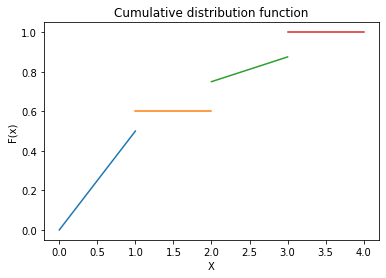
\includegraphics[width=0.55\textwidth]{assignment2.png}
\end{center}
\end{figure}

\end{document}

